\documentclass[12pt]{article}
\usepackage{amsmath}
\usepackage{gensymb}
\usepackage{float}
\usepackage[top=1.25in, bottom=1in, left=1in, right=1in]{geometry}
\usepackage{graphicx}
\usepackage[export]{adjustbox}
\usepackage{rotating}
\usepackage{multirow}
\usepackage{latexsym}
\usepackage{amssymb}
\usepackage{longtable}
\usepackage{fancyhdr}
\usepackage{color}
\usepackage{listings}
\usepackage{setspace}
\definecolor{Code}{rgb}{0,0,0}
\definecolor{Decorators}{rgb}{0.5,0.5,0.5}
\definecolor{Numbers}{rgb}{0.5,0,0}
\definecolor{MatchingBrackets}{rgb}{0.25,0.5,0.5}
\definecolor{Keywords}{rgb}{0,0,1}
\definecolor{self}{rgb}{0,0,0}
\definecolor{Strings}{rgb}{0,0.63,0}
\definecolor{Comments}{rgb}{0,0.63,1}
\definecolor{Backquotes}{rgb}{0,0,0}
\definecolor{Classname}{rgb}{0,0,0}
\definecolor{FunctionName}{rgb}{0,0,0}
\definecolor{Operators}{rgb}{0,0,0}
\definecolor{Background}{rgb}{0.98,0.98,0.98}
\lstdefinelanguage{Python}{
	numbers=left,
	numberstyle=\scriptsize ,
	numbersep=1em,
	xleftmargin=1em,
	framextopmargin=2em,
	framexbottommargin=2em,
	showspaces=false,
	showtabs=false,
	showstringspaces=false,
	frame=l,
	tabsize=4,
	% Basic
	basicstyle=\ttfamily\small\setstretch{1},
	backgroundcolor=\color{Background},
	% Comments
	commentstyle=\color{Comments}\slshape,
	% Strings
	stringstyle=\color{Strings},
	morecomment=[s][\color{Strings}]{"""}{"""},
	morecomment=[s][\color{Strings}]{'''}{'''},
	% keywords
	morekeywords={import,from,class,def,for,while,if,is,in,elif,else,not,and,or,print,break,continue,return,True,False,None,access,as,,del,except,exec,finally,global,import,lambda,pass,print,raise,try,assert},
	keywordstyle={\color{Keywords}\bfseries},
	% additional keywords
	morekeywords={[2]@invariant,pylab,numpy,np,scipy},
	keywordstyle={[2]\color{Decorators}\slshape},
	emph={self},
	emphstyle={\color{self}\slshape},
	%
}

\definecolor{mygreen}{rgb}{0,0.6,0}
\definecolor{mygray}{rgb}{0.5,0.5,0.5}
\definecolor{mymauve}{rgb}{0.58,0,0.82}             
\pagestyle{fancy}
\fancyhf{}
\fancyhead[RE,RO]{Zixu Zhang\\zixu@umich.edu}
\fancyhead[LE,LO]{EECS 504\\FALL 2018 }
\fancyhead[C]{Homework 1\textsl{\textsl{}}}

\begin{document}
	\begin{enumerate}
		\item 
		\begin{enumerate}
			\item $$w\begin{bmatrix}
			x'\\y'\\1
			\end{bmatrix}=\begin{bmatrix}
			h_{11} & h_{12} & h_{13}\\
			h_{21} & h_{22} & h_{23}\\
			h_{31} & h_{32} & 1
			\end{bmatrix}\begin{bmatrix}
			x\\y\\1
			\end{bmatrix}=\begin{bmatrix}
			w & 0 & 0\\
			0 & w & 0\\  
			0 & 0 & 2
			\end{bmatrix}\begin{bmatrix}
			x'\\y'\\1
			\end{bmatrix}$$
			
			$$\Rightarrow\begin{bmatrix}
			x'\\y'\\1
			\end{bmatrix}=\begin{bmatrix}
			w & 0 & 0\\
			0 & w & 0\\  
			0 & 0 & 2
			\end{bmatrix}^{-1}\begin{bmatrix}
			h_{11} & h_{12} & h_{13}\\
			h_{21} & h_{22} & h_{23}\\
			h_{31} & h_{32} & 1
			\end{bmatrix}\begin{bmatrix}
			x\\y\\1
			\end{bmatrix}$$
			
			$$\Rightarrow\begin{bmatrix}
			x_i'\\y_i'\\1
			\end{bmatrix}=\begin{bmatrix}
			h_{11}/w & h_{12}/w & h_{13}/w\\
			h_{21}/w & h_{22}/w & h_{23}/w\\
			h_{31}/w & h_{32}/w & 1/w
			\end{bmatrix}\begin{bmatrix}
			x_i\\y_i\\1
			\end{bmatrix}$$
			$$\Rightarrow\begin{cases}
			\frac{h_{11}x_i+h_{12}y_i+h_{13}}{w}=x_i\\
			\frac{h_{21}x_i+h_{22}y_i+h_{23}}{w}=y_i\\
			\frac{h_{31}x_i+h_{31}y_i+h_{33}}{w}=1
			\end{cases}$$
			If we have $n$ pairs of homography data $\{(x_1,y_1),(x_1',y_1')\}$, $\{(x_2,y_2),(x_2',y_2')\},\cdots,$ $\{(x_n,y_n),(x_n',y_n')\}$, we can first construct a sub-matrix $A_{i}$ as 
			$$A_{i}=\begin{bmatrix}
			x_i & y_i & 1 & 0 & 0 & 0 & 0 & 0 & 0\\
			0 & 0 & 0 & x_i & y_i & 1 &  0 & 0 & 0\\
			 0 & 0 & 0 & 0 & 0 & 0 & x_i & y_i & 1 \\
			\end{bmatrix}$$
			
			If we set $x$ as $x=[\frac{h_{11}}{w},\frac{h_{12}}{w},\frac{h_{13}}{w},\frac{h_{21}}{w},\frac{h_{22}}{w},\frac{h_{23}}{w},\frac{h_{31}}{w},\frac{h_{32}}{w},\frac{1}{w}]^T$, we will have
			$$A=\begin{bmatrix}
			A_1\\A_2\\\vdots\\A_n
			\end{bmatrix}\in\mathbb{R}^{3n\times9}, \text{and }\mathbf{y}=\begin{bmatrix}
			x_1'\\y_1'\\1\\\vdots\\x_n'\\y_n'\\1
			\end{bmatrix}\in\mathbb{R}^{3n}$$\\
			
			\item To solve least-square problem $x^*=\operatorname*{argmin}_x||Ax-y||_2$, we can say
			$$x^*=\operatorname*{argmin}_x||Ax-y||_2=\operatorname*{argmin}_x||Ax-y||_2^2$$
			$$\Rightarrow x^*=\operatorname*{argmin}_xE(x), \text{where }E(x)= (Ax-y)^T(Ax-y)= x^TA^TAx-2x^TA^Ty+y^Ty$$
			$$\frac{d}{dx}E(x)=2A^TAx-2A^Ty$$
			Since $E(x)$ is in the quadratic form, it is convex, and its minimum value exists at 
			$$\frac{d}{dx}E(x)=0\Rightarrow A^TAx^*=A^Ty$$
			If $A^TA$ is invertible, the we are able to obtain an unique solution for $x^*$ as
			$$x^*=(A^TA)^{-1}A^Ty$$
			
			To determine if $A^TA$ is invertible, we need to look at the kernel of $A^TA$ as
			$$A^TAx=\vec{0}\Rightarrow x^TA^TAx=\vec{0}\Rightarrow(Ax)^T(Ax)=0$$
			$$\Rightarrow Ax=0\Rightarrow \ker(A^TA)=\ker(A)$$
			$$\because A=\begin{bmatrix}
			x_1 & y_1 & 1 & 0 & 0 & 0 & 0 & 0 & 0\\
			0 & 0 & 0 & x_1 & y_1 & 1 &  0 & 0 & 0\\
			0 & 0 & 0 & 0 & 0 & 0 & x_1 & y_1 & 1 \\
			&&&&\vdots\\
			x_n & y_n & 1 & 0 & 0 & 0 & 0 & 0 & 0\\
			0 & 0 & 0 & x_n & y_n & 1 &  0 & 0 & 0\\
			0 & 0 & 0 & 0 & 0 & 0 & x_n & y_n & 1 \\
			\end{bmatrix}$$
			Thus, we can have following conclusions:(1) If $n<3$ the solution for this least square problem is not unique, since Rank$(A^TA)<9$. There will be infinity solutions for this questions.\\
			(2) If $n\geq 3$ there may have unique solution for this least square problem, given $n$ distinct pairs of points are not aligned with each other. If $n$ distinct pairs of points are not aligned with each other, it is trivial to see that all column vectors in $A$ are linearly independent, Rank$(A^TA)=9$, and $A^TA$ is invertible. \\
					
			\item Partial code in function \texttt{main(n)} is shown as following
			\begin{lstlisting}[language=Python]
yVec = np.ones((3*n)) # vector y
aMat = np.zeros((3*n,9)) # Matrix A

for i in range(n): 
	# form matrix a and y for LR
	yVec[3*i] = XY2[i, 0]
	yVec[3*i+1] = XY2[i, 1]
	aMat[3*i, 0:2] = XY1[i, :]
	aMat[3*i, 2]=1
	aMat[3*i+1, 3:5] = XY1[i, :]
	aMat[3*i+1, 5]=1
	aMat[3*i+2, 6:8] = XY1[i, :]
	aMat[3*i+2, 8]=1

#solve for x*=argmin||Ax-y||_2
ataMatinv = np.linalg.inv((np.matmul(aMat.T,aMat)))
xVec = np.matmul(np.matmul(ataMatinv, aMat.T), yVec)

#Form homogenous transformation matrix 
tMat=np.zeros((3,3))
tMat[0,:]=xVec[0:3]
tMat[1,:]=xVec[3:6]
tMat[2,:]=xVec[6:9]
line1MatHomo = np.array([[u[0],u[1]], \
			[v[0],v[1]],[1,1]], dtype=float)

# calculate corresponding points
line2MatHomo = np.matmul(tMat,line1MatHomo)

# check if new line go out of image
u2Vec = line2MatHomo[0,:]
v2Vec = line2MatHomo[1,:]

# plotting the Fooball image 1 with marker 33
fig2 = plt.figure()
ax2 = fig2.add_subplot(111)
ax2.imshow(img2)
ax2.plot(u2Vec, v2Vec,color='yellow')
ax2.set(title='Football image 2')
ax2.set_adjustable('box-forced')
plt.xlim(0,img2.shape[1])
plt.ylim(0,img2.shape[0])
plt.gca().invert_yaxis()
plt.show()
		\end{lstlisting} 
		\begin{figure}[H]
			\adjincludegraphics[trim={{.1\width} {.05\width} {.1\width} {.05\width}},clip,width=\textwidth]{figure_1}
			\caption{Baseline image with maker 33 highlighted}
			\adjincludegraphics[trim={{.1\width} {.05\width} {.1\width} {.01\width}},clip,width=\textwidth]{figure_2}
			\caption{Output image with maker 33 highlighted}
		\end{figure}
	
		
	
	\end{enumerate}
\item 
\begin{enumerate}
	\item Both persons will observe the reflection with the same intensity. Because according to Lambertian model, the reflectance is independent of reflectance direction $d$.
	
	\item It is not a good model, since it does not work on surface such as metal and mirror. \\
\end{enumerate}

	\item \begin{enumerate}
		\item One way to deal with the boundary vale is zero-padding the image $A$, such that we will have 
		$$\tilde{A}=\begin{bmatrix}
		0 & 0 & 0 & 0\\ 0 & 4 & 8 & 0\\ 0 & 2 & 3 & 0\\ 0 & 1 & 6 & 0\\0 & 0 & 0 & 0
		\end{bmatrix}$$ 
		Or numerically, we can say that $C=A*B$, where 
		$$C(i,j)=\sum_{p=1}^{3}\sum_{q=1}^{2}A(p,q)B(i-p+1,j-q+1)$$
		$$C=\begin{bmatrix}
		4 & 16 & 16\\ 10& 23 & 6\\ 5 & 14 & 12\\ 2 & 12 & 0
		\end{bmatrix}$$
		
		\item Assume the size of image is $m\times n$. Set flipped x-derivative kernel as $k_x=[1,-1]$, and flipped y-derivative kernel as $k_y=[1,-1]$. Whereby, the gradient of image in $x$ and $y$ direction can be expressed as 
		$\nabla I=\begin{bmatrix}
		k_x\otimes I&k_y\otimes I
		\end{bmatrix}^T$, where convolutions are calculated by
\begin{lstlisting}[language=Python]
def _convolve(kernel, in_img):
	kernel_size = kernel.shape
	ker_h = kernel_size[0]
	ker_w = kernel_size[1]
	
	in_img_size = in_img.shape
	img_h = in_img_size[0]
	img_w = in_img_size[1]
	
	out_h = img_h-ker_h+1
	out_w = img_w-ker_w+1
	out_img = np.zeros((out_h, out_w))
	
	for i in range(out_h):
		for j in range(out_w):
			temp=0
			for q in range(ker_w):
				for p in range(ker_h):
					temp += kernel[p,q]*in_img[i+p,j+q]
			
			out_img[i,j] = temp
	return out_img
\end{lstlisting}

We can see that the resultant gradient matrices has dimensions $\nabla_x I\in\mathbb{R}^{m\times (n-1)}$ and $\nabla_y I\in\mathbb{R}^{(m-1)\times n}$. The whole process takes $2m(n-1)$ floating points operations for $\nabla_xI$ and $2(m-1)n$ floating points operations for $\nabla_yI$.\\

After we obtained the gradient matrices, we are able to calculate Potts energy by iterating through two gradient matrices with following codes:
\begin{lstlisting}[language=Python]
def _calculate_potts_energy(data):
	beta = 1
	Ener = 0
	'''
	calculate potts energy in x
	'''
	xdMat = etai.read(data.x_derivative_path)
	for i in range(xdMat.shape[0]):
		for j in range(xdMat.shape[1]):
			if xdMat[i,j] != 0:
				Ener += beta
	'''
	calculate potts energy in y
	'''
	ydMat = etai.read(data.y_derivative_path)
	for i in range(ydMat.shape[0]):
		for j in range(ydMat.shape[1]):
			if ydMat[i,j] != 0:
				Ener += beta
	return Ener
\end{lstlisting} 
	We can see that this operation has $m(n-1)+n(m-1)$ floating points operations. Thus, we can say the the time complexity of this algorithm is $O(n^2)$. Moreover, we get $E(I)=341202$\\
	
	\item After we convolute the original image with a Gaussian kernel, we obtain the new Potts energy $E(I')=155192$.\\
	There is a large difference in Potts energy before and after Gaussian Kernel, since Gaussian filter is a low pass filter that smooths the image and remove some noise. Therefore, after the image convoluted with the Gaussian Kernel, some of pixel changes are removed and Potts energy decreases.\\
	\pagebreak
	\item We found the Potts energy of \texttt{img\_1.jpg} is $E(I_1)=1560$ and Potts energy of \texttt{img\_2.jpg} is $E(I_2)=1560$. Both images have the same Potts energy, since the total length of edge of both images are same.
	\end{enumerate}

	\item \begin{enumerate}
		\item The image $I$ is a $20\times20\times3$ images with RGB colorspace. We can extract $k$-th channel of $I$ with a $3D$ vector whose $k$-th layer is an $20\times20$ identity matrix and other two layers are zeros. Then, we have $I_R,~I_G,~I_B\in\mathbb{I}^{20\times20}$.
		\begin{itemize}
			\item Operation on $I_G$.\\
			The green block has its centroid at $C_G=(6,16)$, it need to rotate by $-90^\circ$ and translate to new centroid $C_G'=(11,10)$. A good choice for transformation matrix is $T_G$:
			$$T_G=\begin{bmatrix}
			0 & 1 & -5\\
			-1 & 0 & 16\\
			0 & 0 & 1
			\end{bmatrix}$$
			Then, we can use use $T_G$ to map every pixel of $I_G$ to new image $I_G'$.
			 \item Operation on $I_B$.\\
			The blue block has its centroid at $C_B=(11,13)$. It need to scale 2 times along $x$-axis and 1.5 times along $y$-axis. Moreover, it needs to translate its centroid to $C_B'=(11,12.5)$. A good choice for transformation matrix is $T_B$:
			$$T_B=\begin{bmatrix}
			2 & 0 & -11\\
			0 & 1.5 & -7\\
			0 & 0 & 1
			\end{bmatrix}$$
			Then, we can use use $T_B$ to map every pixel of $I_B$ to new image $I_B'$.
			Since we do not need any operation on red channel, we can form the new image by stacking $I_R,~I_G',~I_B'$.
		\end{itemize}
	
		\item $T_G$ is an Euclidean transformation.\\
			$T_B$ is an shear transformation.
	\end{enumerate}
	\pagebreak
	\item
	\begin{enumerate}
		\item We first smooth this image with a Gaussian kernel with $\sigma=0.35$. Then, the gradient intensity image is shown in Figure \ref{fig: q4a}
		
		\begin{figure}[H]
			\centering
			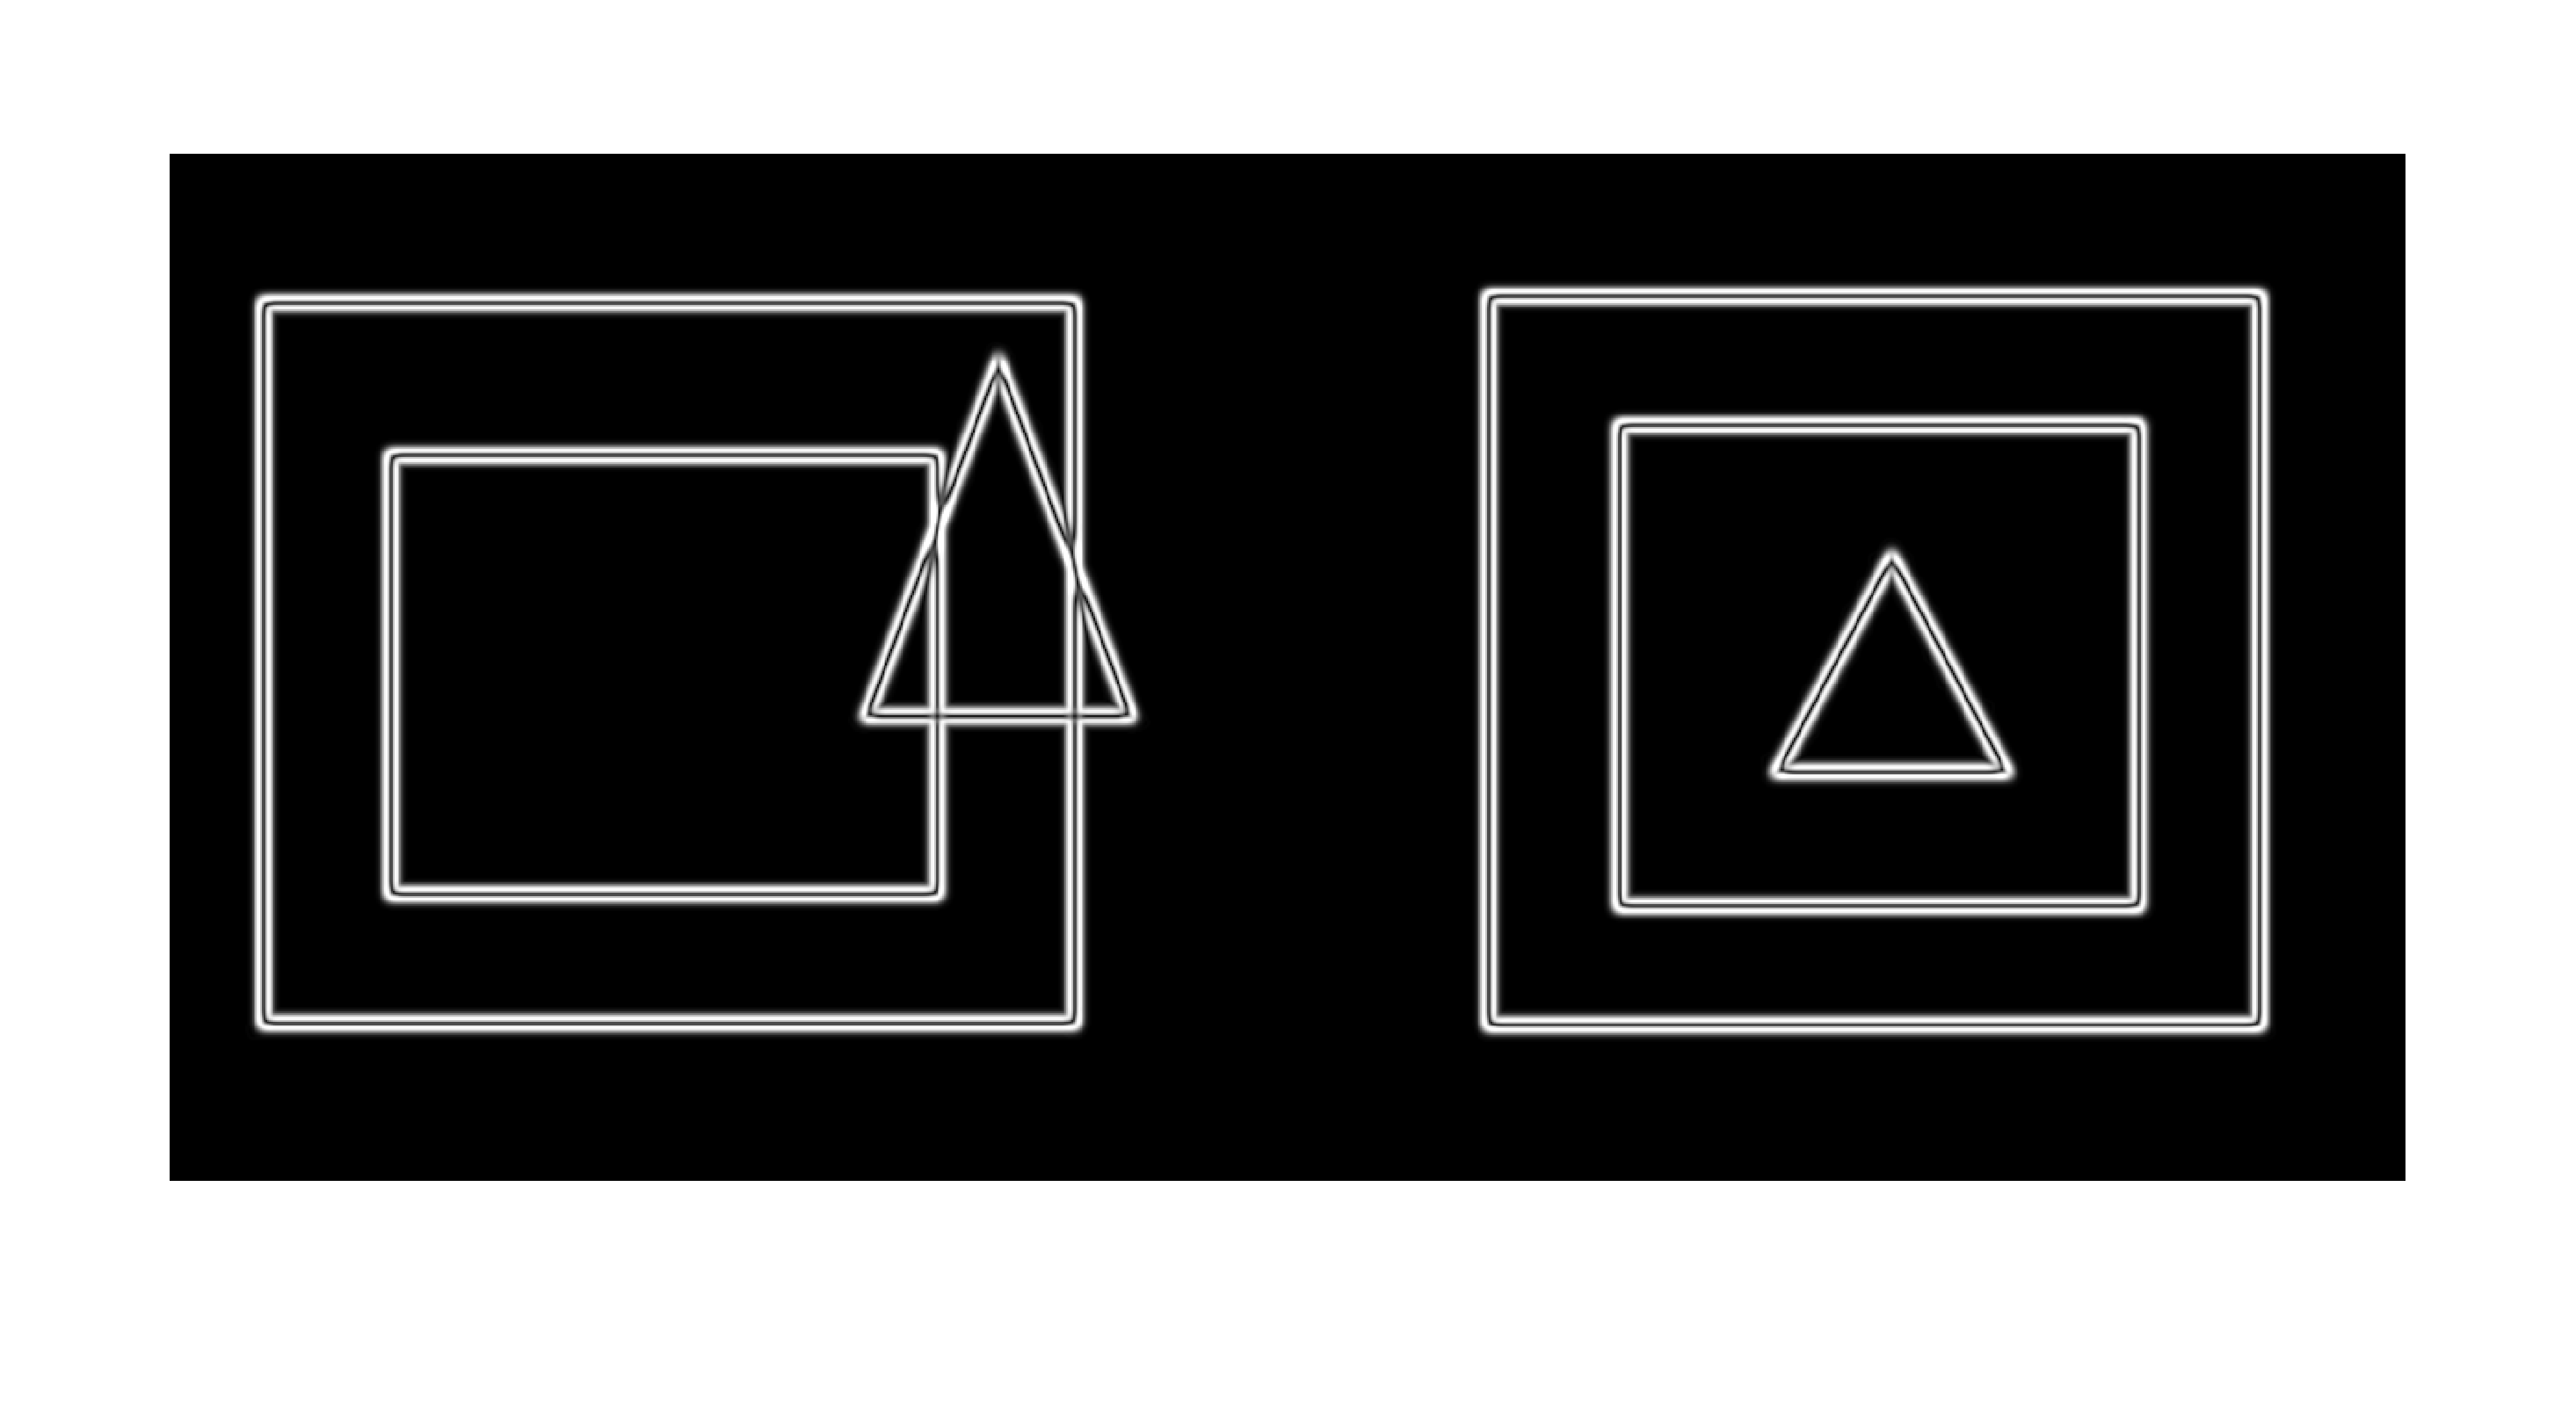
\includegraphics[width=\textwidth]{q4a.eps}
			\vspace{-4em}
			\caption{Gradient intensity of Gaussian smoothed image}\label{fig: q4a}
		\end{figure}
	From this image, we can see that the edge are clear but not sharp. This is caused by Gaussian kernel, which smooths sharp changes in pixels. This leads to thicker edge shown in intensity image and rounded corners.\\
	
\begin{lstlisting}[language=Python]
def _create_sobel_horizontal_kernel():
'''Creates the 3x3 horizontal sobel kernel.
Returns:
kernel: the sobel horizontal kernel
'''
	return np.array([[1,0,-1],[2,0,-2],[1,0,-1]])


def _create_sobel_vertical_kernel():
'''Creates the 3x3 vertical sobel kernel.
Returns:
kernel: the sobel vertical kernel
'''
	return np.array([[1,2,1],[0,0,0],[-1,-2,-1]])
	
def _convolve(kernel, in_img):
'''Convolve the input image "in_img" with the kernel "kernel".
Assume the kernel has already been flipped.

Args:
kernel: a 2d kernel that is assumed to be flipped appropriately
in_img: the input image

Returns:
out_img: the result of convolving the input image with the specified
kernel
'''
	'''get kernel size'''
	kernel_size = kernel.shape
	ker_h = kernel_size[0]
	ker_w = kernel_size[1]
	
	'''get input size'''
	in_img_size = in_img.shape
	img_h = in_img_size[0]
	img_w = in_img_size[1]
	
	'''calculate output size'''
	out_h = img_h-ker_h+1
	out_w = img_w-ker_w+1
	
	'''init output image'''
	out_img = np.zeros((out_h, out_w))
	
	for i in range(out_h):
		for j in range(out_w):
		'''loop every centroid'''
			temp=0
			for q in range(ker_w):
				for p in range(ker_h):
				'''element wise multiplication and sum'''
					temp += kernel[p,q]*in_img[i+p,j+q]
					out_img[i,j] = temp
	return out_img
\end{lstlisting}

\pagebreak
	\item After non-maximum suppression, detected edges are shown as Figure \ref{fig: q4b}. Code is listed in Appendix.
	\begin{figure}[H]
		\centering
		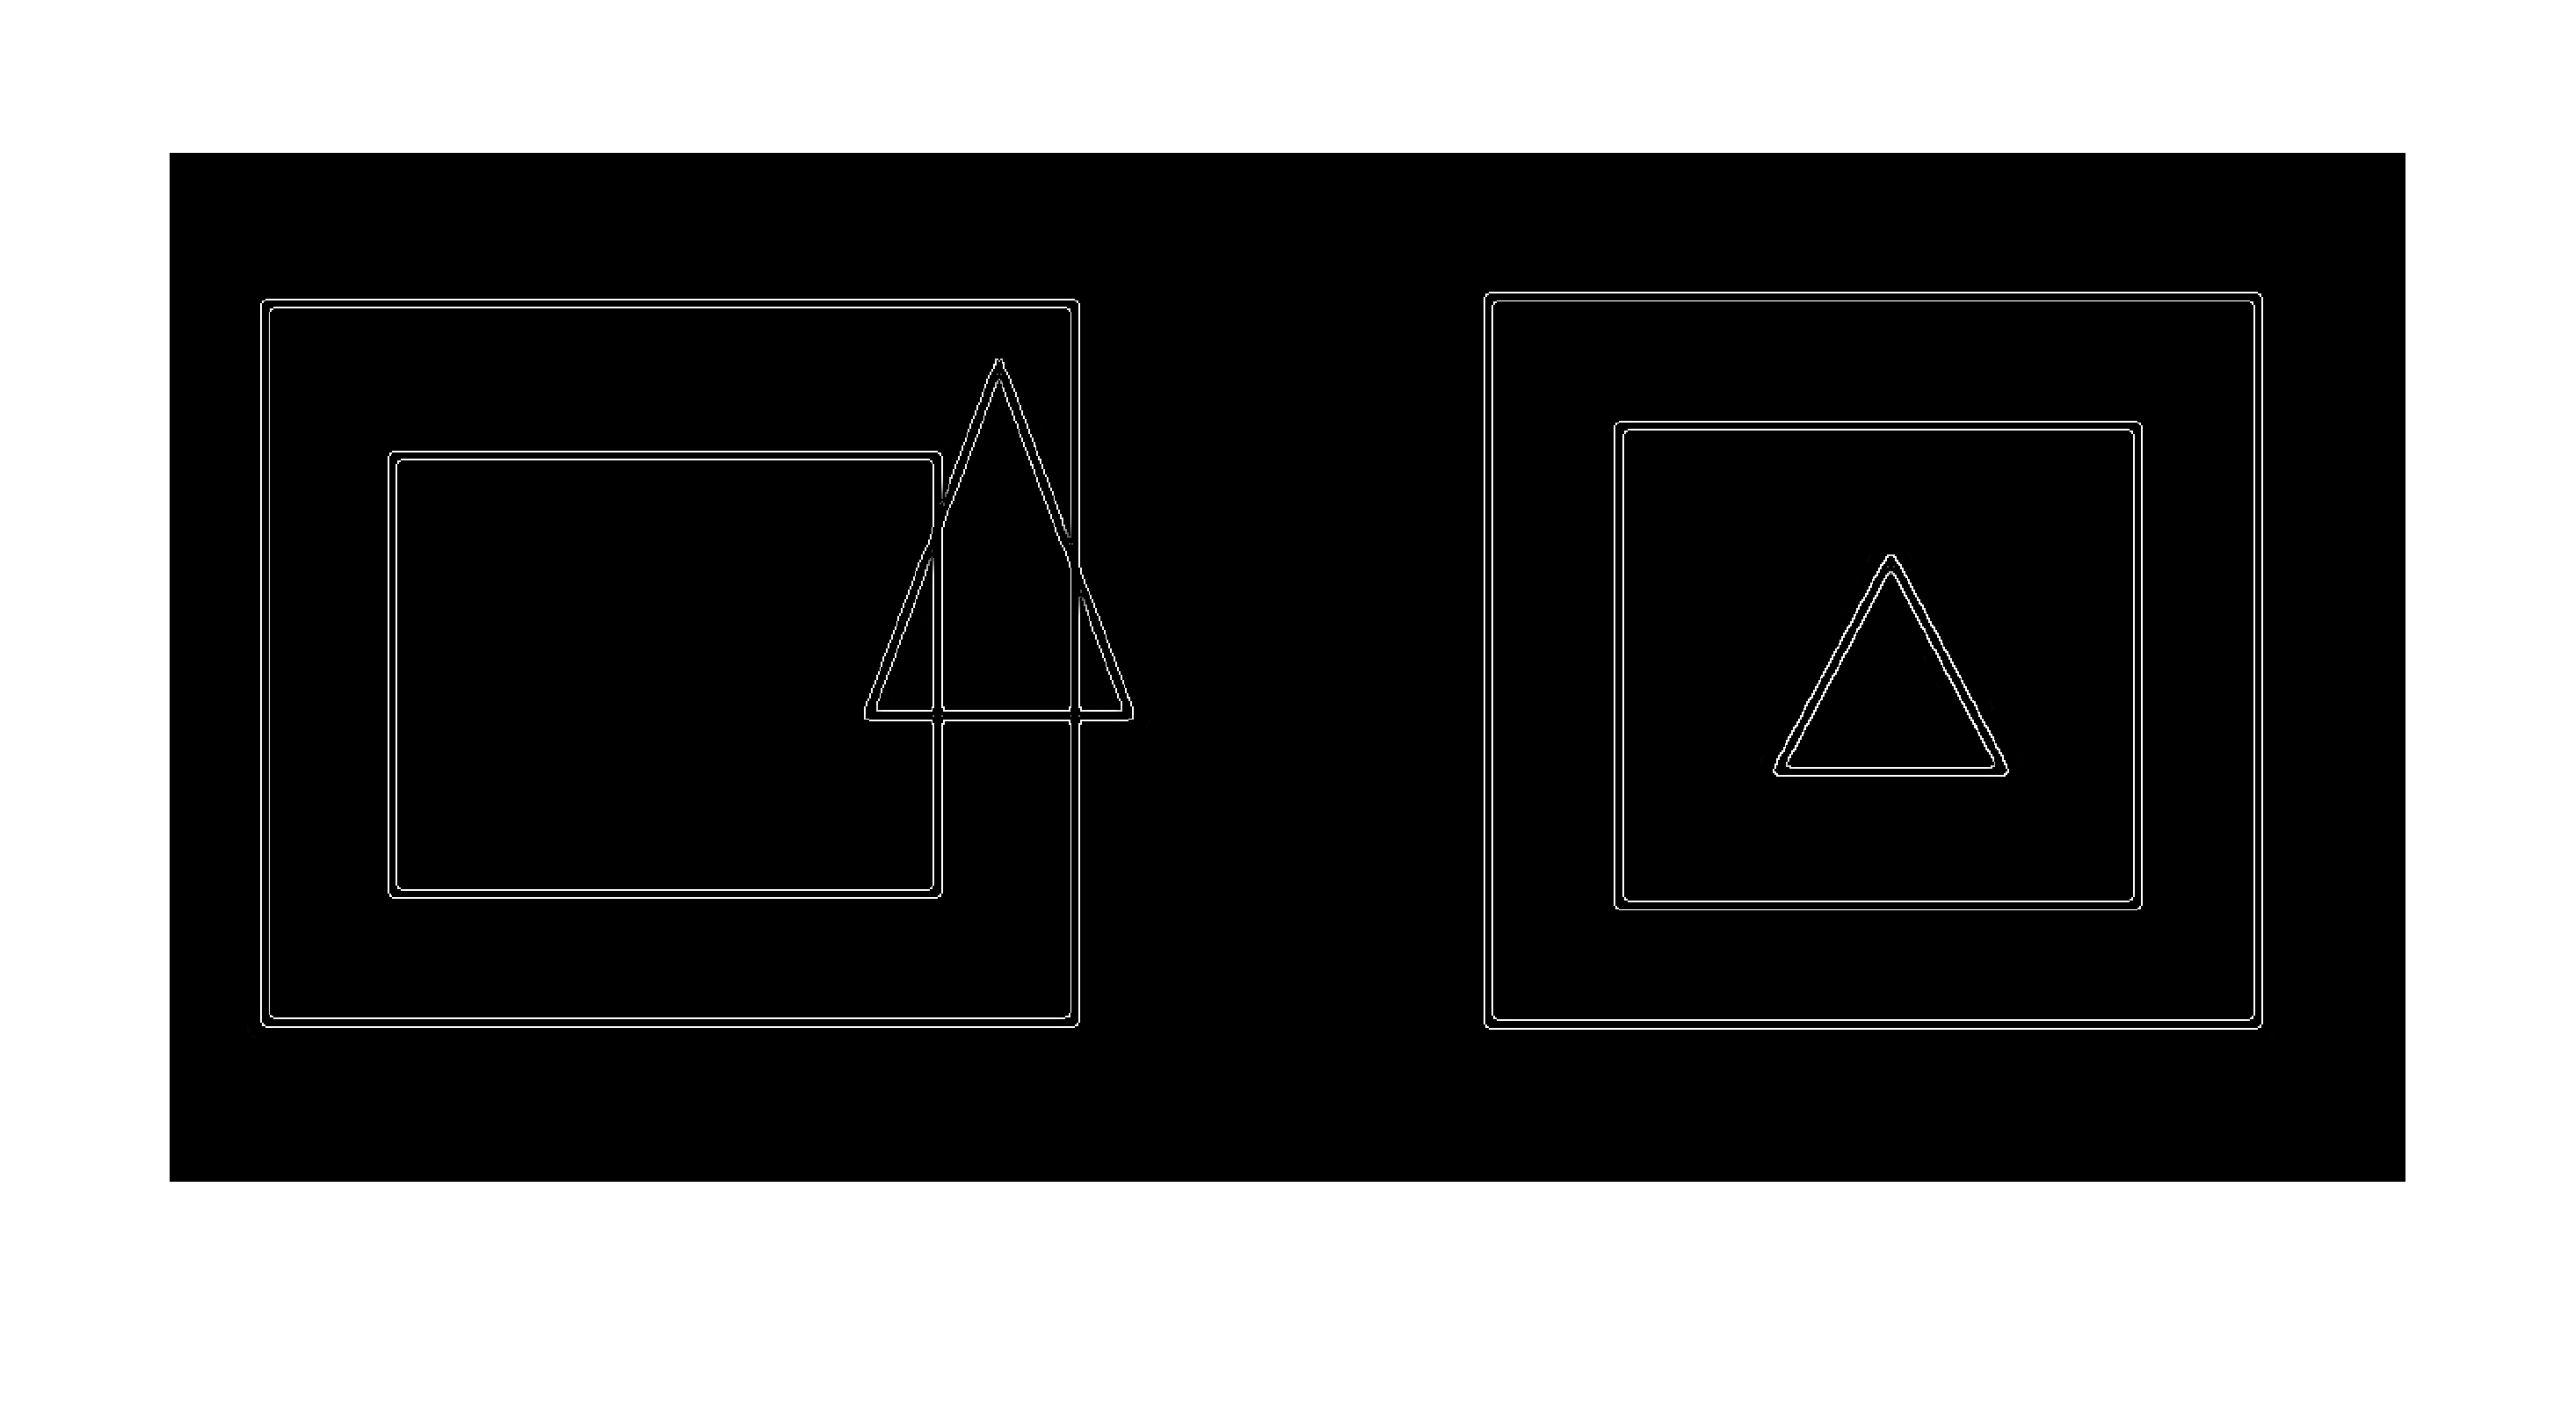
\includegraphics[width=\textwidth]{q4b.eps}
		\vspace{-4em}
		\caption{Detected edges after non-maximum suppression}\label{fig: q4b}
	\end{figure}	
	\item After double threshold and hysteresis, detected edges are shown as Figure \ref{fig: q4c}. Code is listed in Appendix.
	\begin{figure}[H]
		\centering
		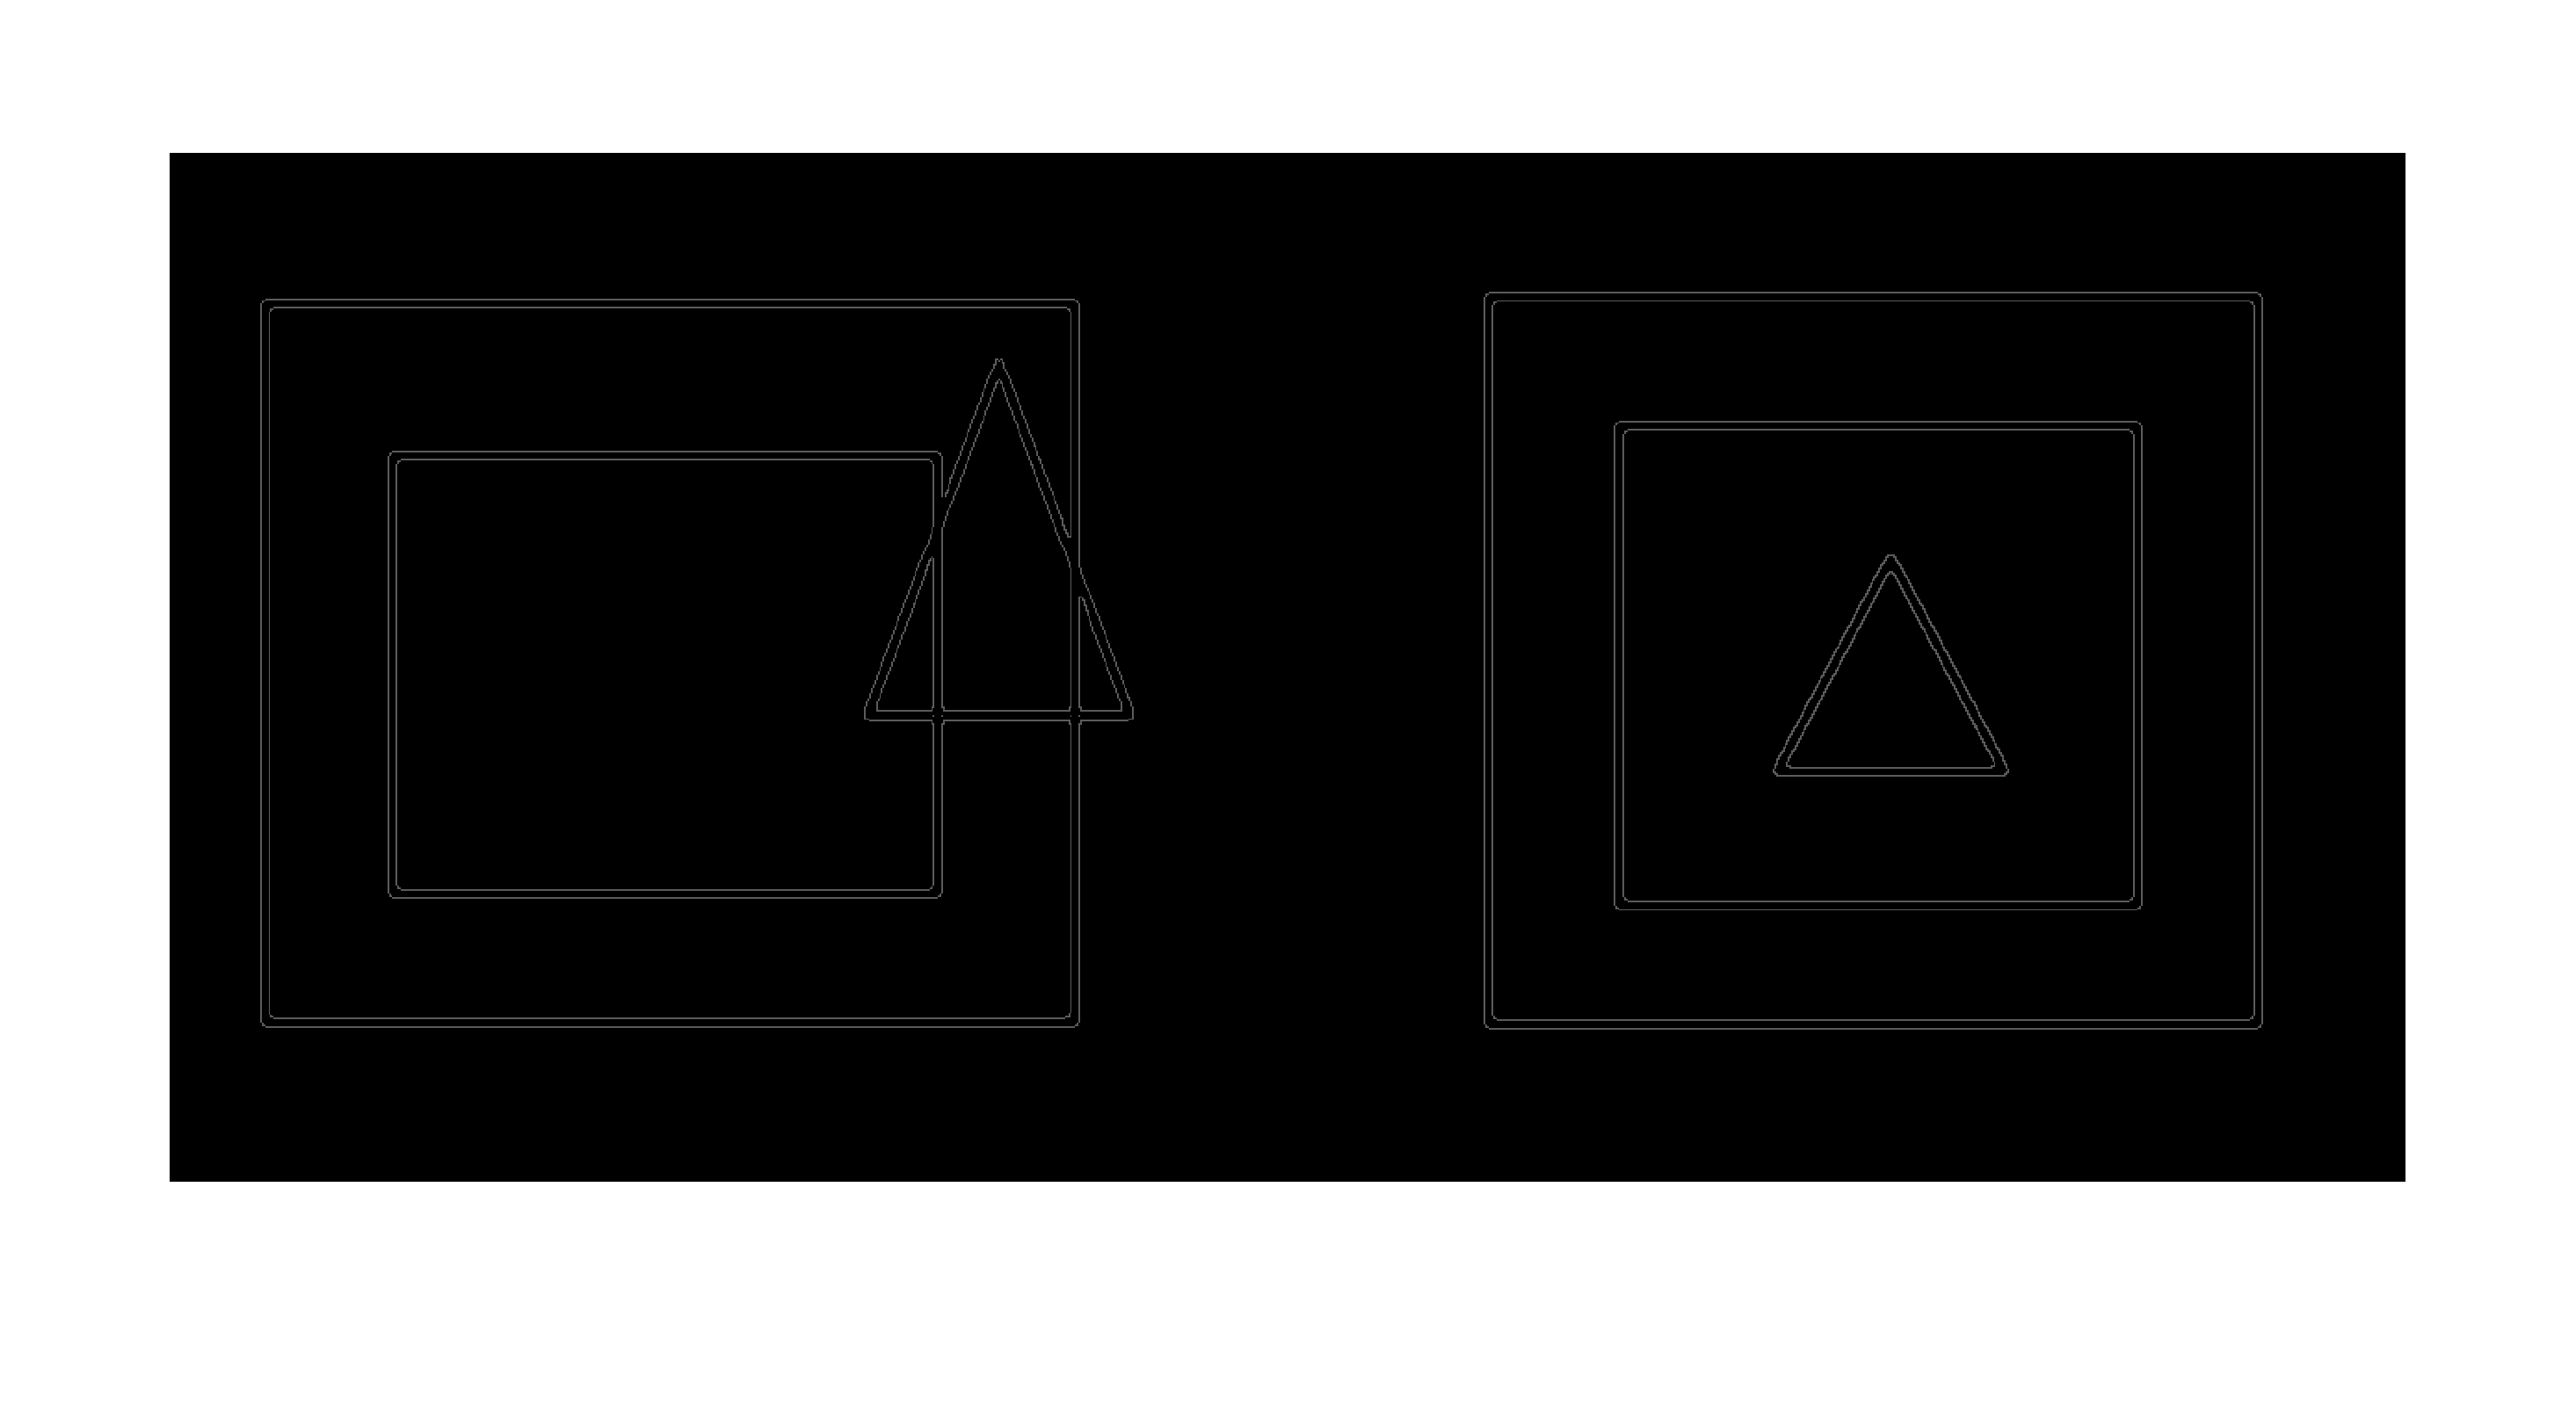
\includegraphics[width=\textwidth]{q4c.eps}
		\vspace{-4em}
		\caption{Detected edges after non-maximum suppression}\label{fig: q4c}
	\end{figure}
\pagebreak

	\item No. The canny edge detector do not have rotation invariance, since the Sobel Operator that obtains image gradient is not an rotational invariant operator. If we look at the Fourier domain of Sobel operator as figure below.
	\begin{figure}[H]
		\centering
		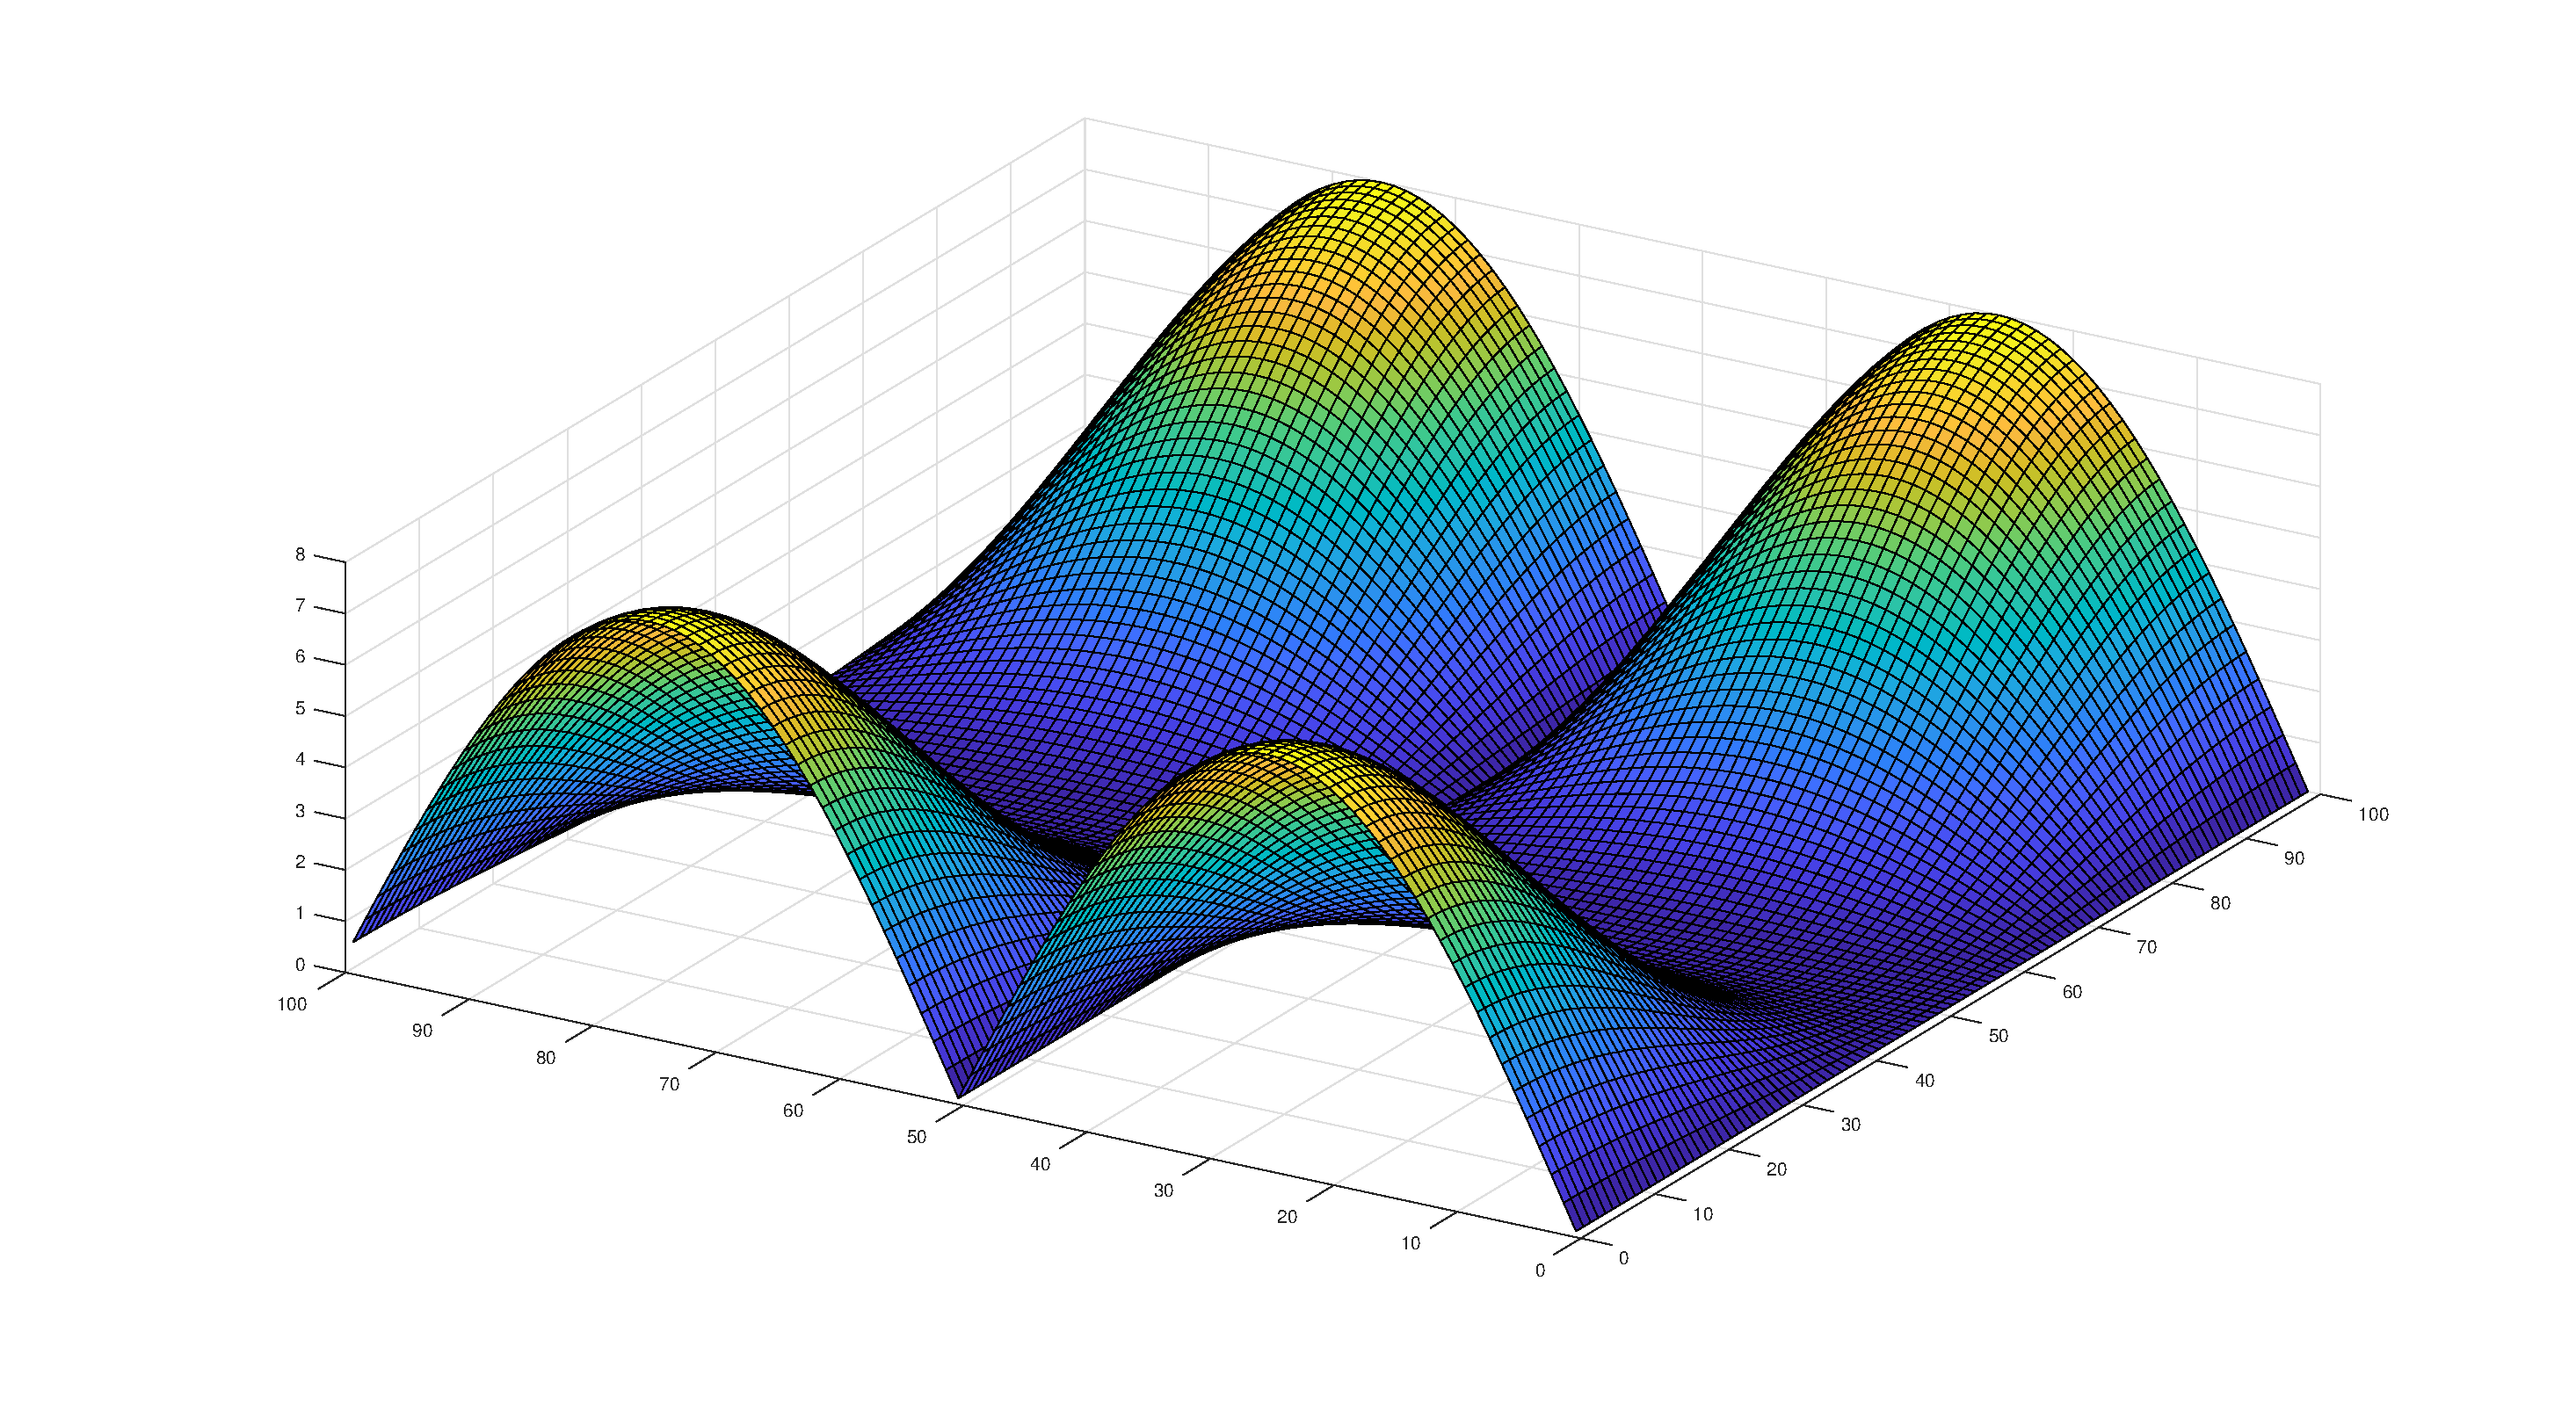
\includegraphics[width=\textwidth]{q4d.eps}
	\end{figure}  
	It is clear the Sobel operator is not symmetric in frequency domain. However, during Fourier transform, rotation in spatial domain also preserves in Fourier domain. This means if we rotate the image, then the spectrum in Fourier domain also rotates by the same amount. However, since convolution is the element-wise product in Fourier domain, results of convolution will differ after rotation. Although, we square the gradients in $x$ and $y$ direction to reduce this effect, and rotation will not change edge detection results by a lot. It is still variant under rotation.\\
	
	\item By using Hough Line Detector, we are able to detect lines in the edge output. After that a naive search along detected lines will help us to find line segments. The results are shown in figure below, where all line segments are highlighted with different colors.
	\begin{figure}[H]
		\centering
		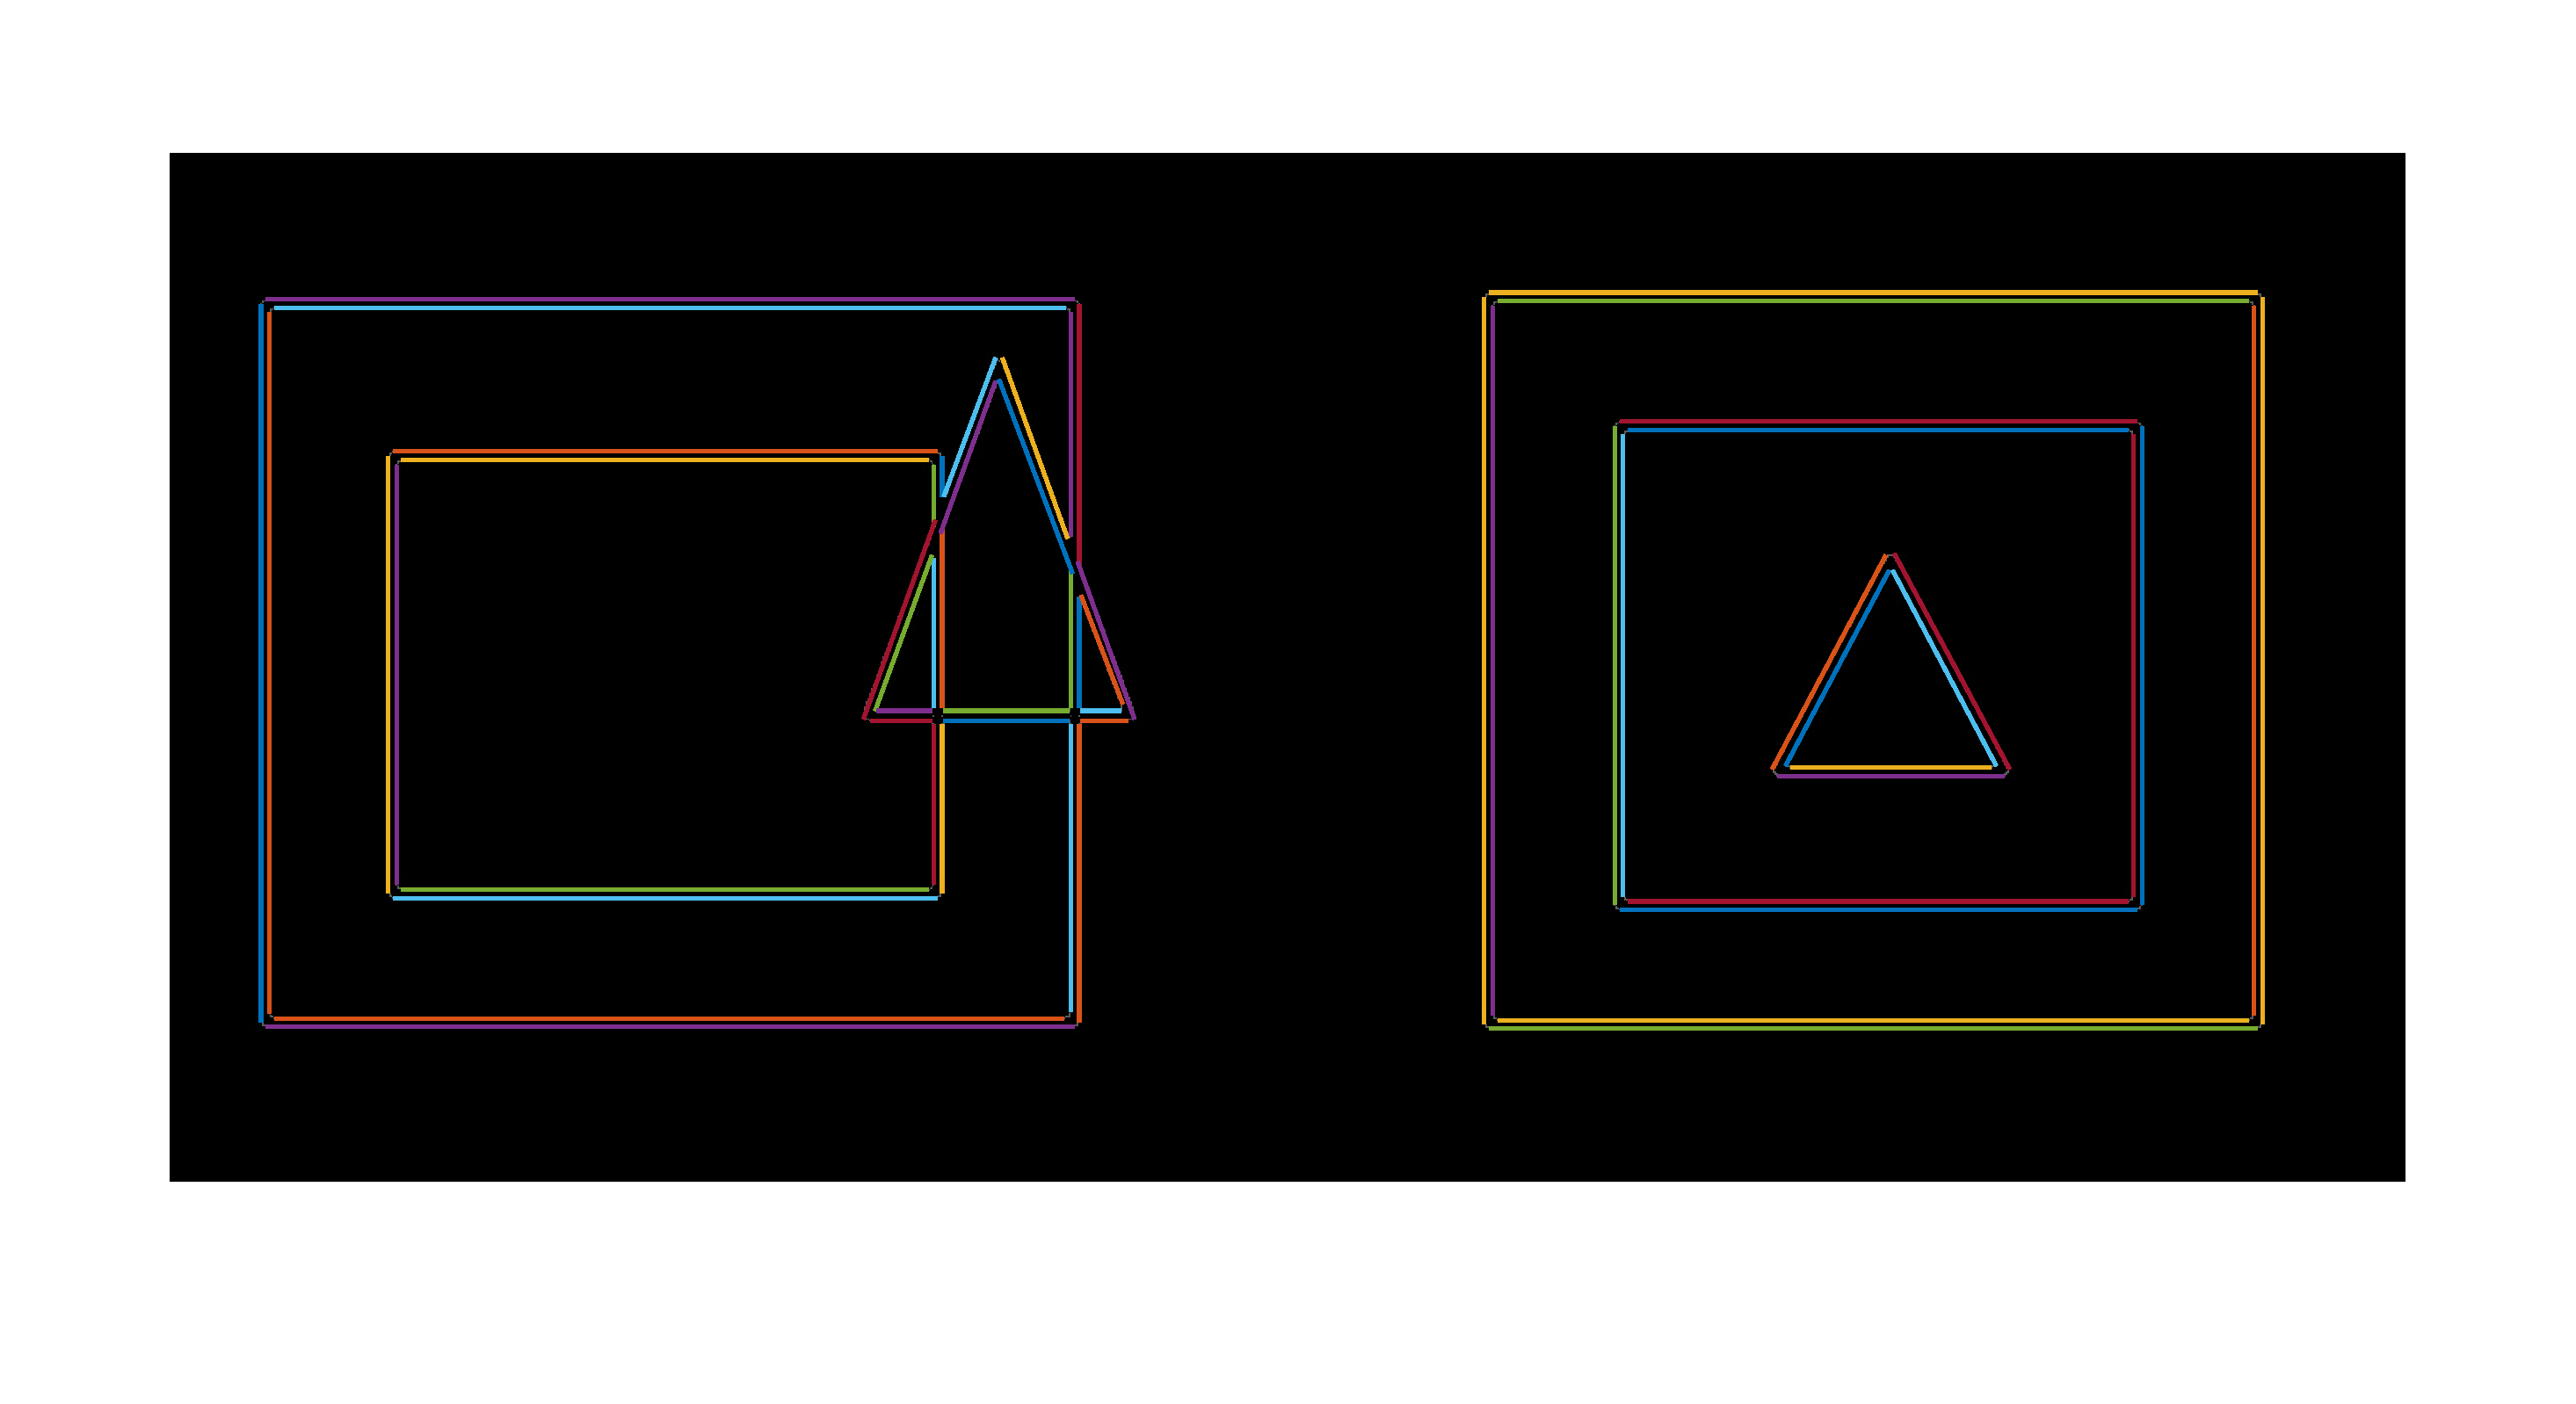
\includegraphics[width=\textwidth]{q4e.eps}
		\vspace{-4em}
	\end{figure} 
	Here is the list of end points of all 60 line segments 
	%\begin{table}[H]
		%\centering
		\begin{longtable}{|c|c|c|c|}
			\hline
			$x$  & $y$ & $x'$ & $y'$ \\ \hline
			55   & 91  & 55   & 520  \\ \hline
			60   & 96  & 60   & 515  \\ \hline
			131  & 182 & 131  & 443  \\ \hline
			136  & 187 & 136  & 438  \\ \hline
			457  & 187 & 457  & 224  \\ \hline
			457  & 243 & 457  & 332  \\ \hline
			457  & 342 & 457  & 438  \\ \hline
			462  & 182 & 462  & 206  \\ \hline
			462  & 225 & 462  & 332  \\ \hline
			462  & 342 & 462  & 443  \\ \hline
			539  & 96  & 539  & 230  \\ \hline
			539  & 249 & 539  & 332  \\ \hline
			539  & 342 & 539  & 514  \\ \hline
			544  & 91  & 544  & 248  \\ \hline
			544  & 266 & 544  & 332  \\ \hline
			544  & 342 & 544  & 520  \\ \hline
			786  & 87  & 786  & 521  \\ \hline
			791  & 92  & 791  & 516  \\ \hline
			864  & 164 & 864  & 450  \\ \hline
			869  & 169 & 869  & 445  \\ \hline
			1174 & 169 & 1174 & 445  \\ \hline
			1179 & 164 & 1179 & 450  \\ \hline
			1246 & 92  & 1246 & 516  \\ \hline
			1251 & 87  & 1251 & 521  \\ \hline
			494  & 137 & 461  & 228  \\ \hline
			456  & 241 & 422  & 334  \\ \hline
			494  & 123 & 463  & 206  \\ \hline
			458  & 220 & 415  & 339  \\ \hline
			1028 & 250 & 966  & 367  \\ \hline
			1026 & 241 & 958  & 369  \\ \hline
			789  & 84  & 1248 & 84   \\ \hline
			58   & 88  & 541  & 88   \\ \hline
			794  & 89  & 1243 & 89   \\ \hline
			63   & 93  & 536  & 93   \\ \hline
			867  & 161 & 1176 & 161  \\ \hline
			872  & 166 & 1171 & 166  \\ \hline
			134  & 179 & 459  & 179  \\ \hline
			139  & 184 & 454  & 184  \\ \hline
			423  & 334 & 456  & 334  \\ \hline
			463  & 334 & 538  & 334  \\ \hline
			545  & 334 & 569  & 334  \\ \hline
			419  & 340 & 456  & 340  \\ \hline
			463  & 340 & 538  & 340  \\ \hline
			545  & 340 & 573  & 340  \\ \hline
			969  & 368 & 1089 & 368  \\ \hline
			961  & 373 & 1097 & 373  \\ \hline
			139  & 441 & 454  & 441  \\ \hline
			134  & 446 & 459  & 446  \\ \hline
			872  & 448 & 1171 & 448  \\ \hline
			867  & 453 & 1176 & 453  \\ \hline
			63   & 518 & 535  & 518  \\ \hline
			794  & 519 & 1243 & 519  \\ \hline
			58   & 523 & 541  & 523  \\ \hline
			789  & 524 & 1248 & 524  \\ \hline
			1030 & 250 & 1092 & 367  \\ \hline
			1031 & 240 & 1100 & 369  \\ \hline
			496  & 136 & 540  & 252  \\ \hline
			545  & 265 & 570  & 330  \\ \hline
			498  & 123 & 537  & 231  \\ \hline
			543  & 245 & 577  & 339  \\ \hline
		\end{longtable}
	%\end{table}

	\end{enumerate}
	\end{enumerate}
\pagebreak
\textbf{Non Maximum Suppression }
\begin{lstlisting}[language=Python]
def _choose_orientation_mode( theta ):
'''
mode 0: -pi/8 < theta <=  pi/8 U theta > 7/8pi 
		U theta<= -7/8pi check horiz
mode 1:  pi/8 < theta <= 3pi/8 U -7pi/8 < theta <= -5pi/8
		 check 1,3 quad
mode 2: 3pi/8 < theta <= 5pi/8 U -5pi/8 < theta <= -3pi/8 
		check vertical
mode 3: 5pi/8 < theta <= 7pi/8 U -3pi/8 < theta <= -pi/8 
		check 2,4 quad
'''
mode = 0
if (-np.pi/8 < theta and theta <= np.pi/8) or theta > 7*np.pi/8 
	or theta <= -7*np.pi/8:
	mode = 0 
elif (np.pi/8 < theta and theta <= 3*np.pi/8) 
	or (-7*np.pi/8 < theta and theta <= -5*np.pi/8):
	mode = 1
elif (3*np.pi/8 < theta and theta <= 5*np.pi/8) 
	or (-5*np.pi/8 < theta and theta <= -3*np.pi/8):
	mode = 2
elif (5*np.pi/8 < theta and theta <= 7*np.pi/8) 
	or (-3*np.pi/8 < theta and theta <= -np.pi/8):
	mode = 3
return mode


def _non_maximum_suppression(g_intensity, orientation, input_image):
	'''Performs non-maximum suppression. If a pixel is not a local maximum
	(not bigger than it's neighbors with the same orientation), then
	suppress that pixel.
	
	Args:
	g_intensity: the gradient intensity of each pixel
	orientation: the gradient orientation of each pixel
	input_image: the input image
	
	Returns:
	g_sup: the gradient intensity of each pixel, with some intensities
	suppressed to 0 if the corresponding pixel was not a local
	maximum
	'''
	input_H = input_image.shape[0]
	input_W = input_image.shape[1]
	
	outputImg = np.zeros((input_H,input_W))
	'''y of pixel corresponding to gradient(0,0)'''
	kernel_H_2 = int((input_H-g_intensity.shape[0])/2) 
	'''x of pixel corresponding to gradient(0,0)'''
	kernel_W_2 = int((input_W-g_intensity.shape[1])/2) 
	
	for i in range(g_intensity.shape[0]): #vertical(y)
		for j in range(g_intensity.shape[1]): #horizontal(x)
			if(g_intensity[i, j]>0):
				'''determine gradient direction'''
				cur_mode = _choose_orientation_mode(orientation[i,j])
				if cur_mode == 0:
					prev_x = j-1
					prev_y = i
					next_x = j+1
					next_y = i
				elif cur_mode == 1:
					prev_x = j-1
					prev_y = i-1
					next_x = j+1
					next_y = i+1
				elif cur_mode == 2:
					prev_x = j
					prev_y = i-1
					next_x = j
					next_y = i+1
				elif cur_mode == 3:
					prev_x = j-1
					prev_y = i+1
					next_x = j+1
					next_y = i-1
				cur_bool = True 
				'''boolen to check if need to perserve'''
				'''check both side along gradient'''
				if prev_x>=0 and prev_x<g_intensity.shape[1] 
					and prev_y>=0 and prev_y<g_intensity.shape[0]:
					if(g_intensity[prev_y,prev_x]>g_intensity[i,j]):
						cur_bool=False
				if next_x>=0 and next_x<g_intensity.shape[1] 
					and next_y>=0 and next_y<g_intensity.shape[0]:
					if(g_intensity[next_y,next_x]>g_intensity[i,j]):
						cur_bool=False
				if cur_bool:
					outputImg[i+kernel_H_2,j+kernel_W_2] 
							= g_intensity[i, j]    
	return outputImg

\end{lstlisting}

\pagebreak
\textbf{Double Thresholding \& Hysteresis}
\begin{lstlisting}[language=Python]
def _double_thresholding(g_suppressed, low_threshold, high_threshold):
'''Performs a double threhold. All pixels with gradient intensity larger
than 'high_threshold' are considered strong edges, all pixels with gradient
intensity in between 'high_threshold' and 'low_threshold' are considered
weak edges, and all pixels with gradient intensity smaller than
'low_threshold' are suppressed to 0.

Args:
g_suppressed: the gradient intensities of all pixels, after
non-maxiumum suppression
low_threshold: the lower threshold in double thresholding
high_threshold: the higher threshold in double thresholding

Returns:
g_thresholded: the result of double thresholding
'''
	'''initialize the image'''
	g_thresholded = np.zeros((g_suppressed.shape[0],
		g_suppressed.shape[1]))
	for i in range(g_thresholded.shape[0]):
		for j in range(g_thresholded.shape[1]):
			if g_suppressed[i,j]<low_threshold:
				g_thresholded[i,j]=0
			elif g_suppressed[i,j]>high_threshold:
				g_thresholded[i,j]=high_threshold
			else:
				g_thresholded[i,j]=low_threshold
	return g_thresholded


def _hysteresis(g_thresholded, low_threshold, high_threshold):
'''Performs hysteresis. If a weak pixel is connected to a strong pixel,
then the weak pixel is marked as strong. Otherwise, it is suppressed.
The result will be an image with only strong pixels.

Args:
g_thresholded: the result of double thresholding

Returns:
g_strong: an image with only strong edges
'''
	g_strong = np.zeros((g_thresholded.shape[0],g_thresholded.shape[1]))
	for i in range(1, g_thresholded.shape[0]-1):
		for j in range(1, g_thresholded.shape[1]-1):
			if g_thresholded[i,j]==high_threshold:
				g_strong[i,j]=high_threshold
				elif g_thresholded[i,j]==low_threshold: 
				''' low threshold'''
					if (g_thresholded[i,j-1]==high_threshold 
						or g_thresholded[i,j+1]==high_threshold 
						or g_thresholded[i+1,j]==high_threshold 
						or g_thresholded[i-1,j]==high_threshold 
						or g_thresholded[i+1,j+1]==high_threshold 
						or g_thresholded[i+1,j-1]==high_threshold
						or g_thresholded[i-1,j+1]==high_threshold 
						or g_thresholded[i-1,j-1]==high_threshold):
						'''check all direction'''
						g_strong[i,j] = high_threshold
					else:
						g_strong[i,j]=0
	return g_strong
	
	
	

		
\end{lstlisting}
	
\end{document}